% Copyright 2015 by Angelos Drossos <angelos.drossos@gmail.com>
%
% This file may be distributed and/or modified
%
% 1. under the LaTeX Project Public License and/or
% 2. under the GNU Public License.
%
% See the file doc/licenses/LICENSE for more details.


\documentclass[%
	english,  % load babel with language english
	%ngerman, % load babel with language ngerman
	]{beamer}
\usepackage{ifluatex}
\ifluatex
\usepackage[%
	%math,    % load math packages
	]{fontspec}
\defaultfontfeatures{%
	Ligatures=TeX
	}
\setmainfont{Linux Libertine O}     % main font
\setsansfont{Linux Biolinum O}      % sans font (for sections)
\setmonofont{Linux LibertineMono O} % mono font (for listings)
\usepackage[%
	protrusion=true, %
	expansion,       %
	]{microtype}
\else
\usepackage[T1]{fontenc}
\usepackage[utf8]{inputenc}
\usepackage[mono=true]{libertine} % main/sans/mono font (Libertine, Biolinum, LibertineMono)
\usepackage[%
	protrusion=true, %
	expansion,       %
	]{microtype}
\fi

\usetheme{Angel707}
%\usetheme{default}

\title[Beamer Theme]{Custom Beamer Template with TikZ -- This is an example presentation}
%\subtitle{}
\author[A.~Drossos]{Angelos Drossos}
\institute[TU]{Technische Universität}
%\date{} % if no date is specified, today is used
\titlegraphic{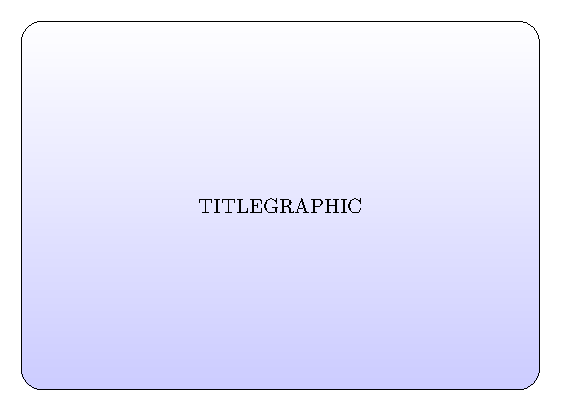
\includegraphics[height=4cm]{titlegraphic.pdf}}
\logo{
\includegraphics[height=0.8cm]{logo.pdf}}
\subject{Beamer Templates with TikZ}
\keywords{LaTeX, Beamer, TikZ}

\begin{document}
\frame[plain]{\titlepage}
%\frame{\titlepage}

\section*{Outline}
\begin{frame}{Outline}
	\tableofcontents[hideallsubsections]
\end{frame}


\section{Introduction}

\begin{frame}{\secname{}}
	\tableofcontents[currentsection,currentsubsection,hideothersubsections]
\end{frame}

\begin{frame}{I am a frame title -- and that is good so}
Hallo, I am a text inside a frame.

\vfill

\begin{itemize}
\item and I am a text inside an itemize environment
\item and a second text
\item and more\ldots
\end{itemize}
\end{frame}


\begin{frame}{I am a frame title -- and that is good so}{And I am a subtitle.. bah!}
Hallo, I am a text inside a frame.

\vfill

\begin{itemize}
\item and I am a text inside an itemize environment
\item and a second text
\item and more\ldots
\end{itemize}
\end{frame}


\section{Bla Bli Blubb Blocks}

\begin{frame}{\secname{}}
	\tableofcontents[currentsection,currentsubsection,hideothersubsections]
\end{frame}

\subsection{Blocks without headers}

\begin{frame}{Blocks}{without headers}
\begin{block}{}
\begin{itemize}
\item and I am a text inside an itemize environment
\item and a second text
\item and more\ldots
\end{itemize}
\end{block}

\vfill

\begin{exampleblock}{}
\begin{itemize}
\item and I am a text inside an itemize environment
\item and a second text
\item and more\ldots
\end{itemize}
\end{exampleblock}

\vfill

\begin{alertblock}{}
\begin{itemize}
\item and I am a text inside an itemize environment
\item and a second text
\item and more\ldots
\end{itemize}
\end{alertblock}
\end{frame}


\subsection{Blocks with headers}

\begin{frame}{Blocks}{with headers}
\begin{block}{a fact}
\begin{itemize}
\item and I am a text inside an itemize environment
\item and a second text
\end{itemize}
\end{block}

\vfill

\begin{exampleblock}{an example}
\begin{itemize}
\item and I am a text inside an itemize environment
\item and a second text
\end{itemize}
\end{exampleblock}

\vfill

\begin{alertblock}{An Alert!!}
\begin{itemize}
\item and I am a text inside an itemize environment
\item and a second text
\end{itemize}
\end{alertblock}
\end{frame}


\section{Overlays}

\begin{frame}{\secname{}}
	\tableofcontents[currentsection,currentsubsection,hideothersubsections]
\end{frame}

\begin{frame}{I am a frame title -- and that is good so}{And I am a subtitle.. bah!}
Hallo, I am a text inside a frame.

\vfill

\begin{block}{Overlays}
\begin{itemize}
\item<+-> and I am a text inside an itemize environment
\item<+-> and a second text
\item<+-> and more\ldots
\end{itemize}
\end{block}
\end{frame}


\appendix

\begin{frame}{\appendixname{} frame}
	\centering
	\usebeamerfont{title}%
	\usebeamercolor[fg]{structure}%
	\appendixname
\end{frame}

\section{A1}

\begin{frame}{A CDEF}
	A text inside an appendix frame.
\end{frame}

\section{B1}

\begin{frame}{B GHIJK}
	Another text inside an appendix frame.
\end{frame}


\end{document}
